\chapter{Gestaltungslösungen evaluieren}
\label{chapter:evaluation}

Im vorherigen Kapitel wurden einzelne Aspekte der konkreten Implementierung der
Gestaltungslösungen vorgestellt. Im nächsten Schritt sollen die so entwickelten
Softwareteile mit einem Nutzer getestet werden. Dies entspricht dem vierten
Schritt \textit{Gestaltungslösungen aus der Benutzerperspektive evaluieren} im
menschzentrierten Gestaltungsprozess der ISO Norm~\cite{ISO9241}. Christian
Moser erklärt in \textit{User Experience Design} den möglichen Ablauf eines
solchen Usertests wie folgt: \glqq{}Bei Tests mit Benutzern wird den
Testteilnehmern der Kontext anhand des Szenarios erklärt und dann werden die
Aufgaben gestellt. Dabei wird beobachtet, wie gut sie diese mit Hilfe des
Prototyps lösen können.\grqq{}~\cite{moserTesting}. In diesem Fall wird der Test
gemeinsam mit \ipName von der allgemeinen Studienberatung der Universität
Kassel durchgeführt. Gemeinsam haben wir uns eine Stunde Zeit genommen, um das
neu entwickelte Modul zur Terminvereinbarung zu testen. Wir sitzen gemeinsam im
Büro von \ipName und können die Software so direkt an seinem Dienstrechner
testen, um den Nutzungskontext möglichst authentisch zu gestalten.

\section{Durchführung des Usertests}

Der Usertest beginnt damit, dass \ipName die Software Stubegru im Browser
aufruft und den View mit dem neuen Kalendermodul zur Terminvergabe öffnet. Sein
erster Blick fällt auf die Monatsübersicht der Termine im November.

\begin{figure}[H]
    \caption{Monatsübersicht der Termine im November.}
    \centering
    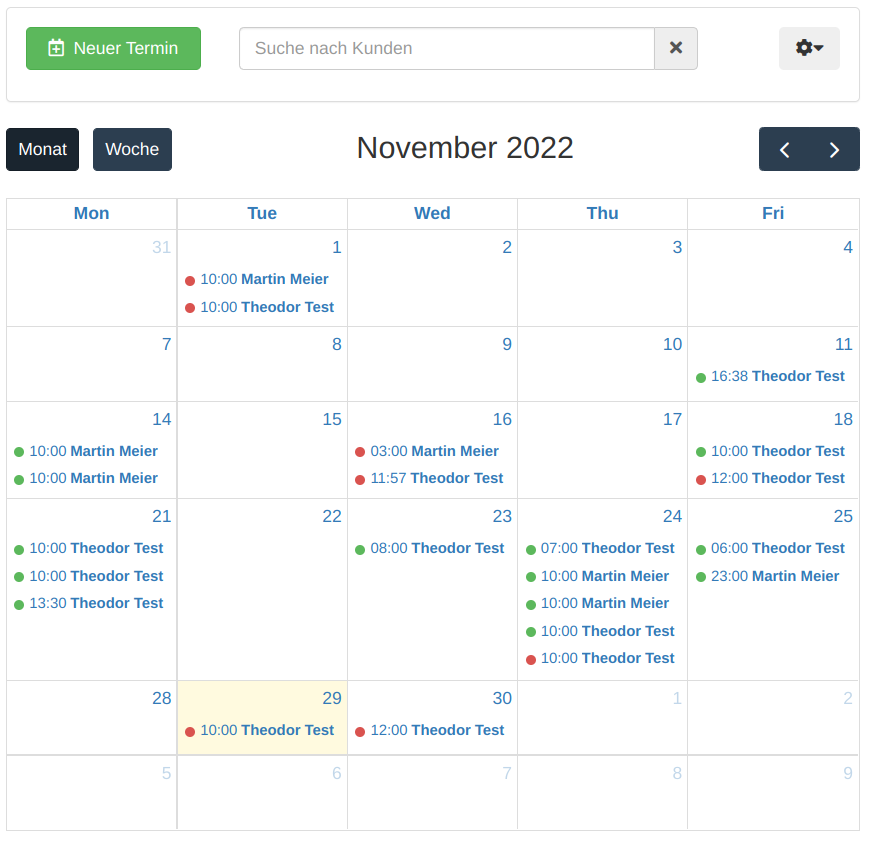
\includegraphics[width=0.9\textwidth]{screen_new_month_view.png}
\end{figure}

In dieser Übersicht kann er einsehen, welche Termine für den aktuellen Monat
eingetragen sind. Anhand der farbigen Punkte kann \ipName auf einen Blick
erkennen, welche Termine noch frei sind und welche bereits an ratsuchende
Kunden vergeben wurden. Neben dem farbigen Punkt kann für jeden Termin
eingesehen werden, bei welchem Studienberatenden dieser Termin stattfindet.
\ipName merkt an, dass es im Vergleich zur alten Version möglich ist, direkt in
der Übersicht zu sehen, zu welchem Zeitpunkt die Termine stattfinden und wie
viele Termine an einem Tag angeboten werden. Er testet, was passiert, wenn viele
Termine am gleichen Tag angelegt werden. Zufrieden stellt er fest, dass die
Zelle für den entsprechenden Tag automatisch größer wird, wenn viele Termine
eingetragen werden. \ipName überlegt weiterhin, dass die Monatsübersicht
dadurch eventuell so lang werden könnte, dass nicht mehr alle Zeilen
gleichzeitig auf den Bildschirm passen könnten. Wir diskutieren, wie viele
Termine üblicherweise pro Tag angeboten werden und einigen uns darauf, die
aktuelle Ansicht zunächst beizubehalten und in der Praxis zu testen.

\begin{figure}[H]
    \caption{Toggles im Dropdown Menü um die angezeigten Termine zu filtern. Hier werden nur freie Termine dargestellt.}
    \centering
    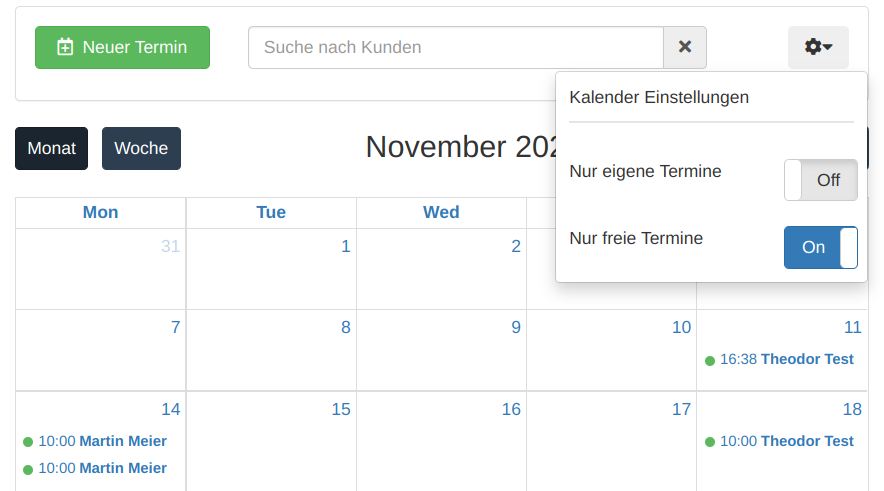
\includegraphics[width=0.9\textwidth]{screen_new_filter.png}
\end{figure}

Ich weise \ipName darauf in, dass er über den Button mit dem Zahnrad weitere
Filtermöglichkeiten hat, um eine überfüllte Monatsübersicht auf die
wesentlichen Termine zu reduzieren. Den Button hat er zunächst nicht bemerkt.
Nachdem er ihn einmal gefunden hat, versteht er die Bedienung über die beiden
Toggles aber schnell. Er merkt positiv an, dass Änderungen an den
Filtereinstellungen direkt übernommen werden und die Auswirkung der Filter
somit leicht zu begreifen ist. Ihm fällt auf, dass der Filter \textit{nur
    eigene Termine anzeigen} für die Hilfskräfte wenig Sinn ergibt, da diese keine
Berechtigung haben, um selber Termine zu erstellen. Sie können lediglich
eingestellte Zeitslots an Ratsuchende vergeben. Wir diskutieren über die
Möglichkeit, diesen Filter für Accounts von Hilfskräften auszublenden,
entscheiden uns aber dafür, dass dies nicht notwendig ist. Der Filter ist für
diese Nutzergruppe zwar überflüssig, aber auch nicht störend.


Als nächstes gebe ich \ipName die Aufgabe, einen neuen Zeitslot zu erstellen.
Ich verrate nicht weiter, wo er diese Funktion finden kann und lasse ihn
ausprobieren. Nach kurzer Zeit entdeckt \ipName den Button \textit{Neuer
    Termin} und es öffnet sich das Modal zum Erstellen eines freien Zeitslots.
\ipName erklärt seine Gedanken: \glqq{}Ich kenne es von anderer Software so,
dass man auf den entsprechenden Tag in der Monatsübersicht klickt, um einen
neuen Termin anzulegen. Aber aus der alten Version von Stubegru erinnere ich
mich noch an den grünen Knopf zum Erstellen eines Termins. Früher war der Knopf
\textit{unter} der Monatsübersicht, aber so fügt er sich elegant in die Leiste
mit der Suche und den neuen Filtern ein.\grqq{}~\cite{clavesUsertest}

\begin{figure}[H]
    \caption{Navigationsleiste über der Monatsansicht. Über den grünen Button kann eine neuer Zeitslot erstellt werden.}
    \centering
    
\includegraphics[width=0.9\textwidth]{screen_new_create_button.png}
\end{figure}

In dem leeren Formular füllt \ipName Schritt für Schritt die Input Felder aus.
Nach einem Klick auf das Feld für die Startzeit ist er enttäuscht. In der alten
Version öffnete sich hier ein \gls{Timepicker}, mit dessen Hilfe man die Uhrzeit
ohne Tastatur nur mit der Maus eingeben konnte. Auch ich bin überrascht, denn
in meinen Tests hatte sich hier auch ein Timepicker geöffnet. Nach kurzer
Recherche stellt sich heraus, dass das verwendete Html5 Input Feld für
Uhrzeiten in jedem Browser unterschiedlich dargestellt
wird~\cite{htmlTimeInput}. Während der Implementierung habe ich die Ergebnisse
immer in \textit{Google Chrome} getestet, dort erscheint nach dem Klick in ein
Uhrzeit-Input ein Timepicker. Die Abteilung der Studienberatung verwendet in
der Regel Firefox als Browser, da dieser auf den Dienstrechnern standardmäßig
vorinstalliert ist. Ich verspreche, mich dem Problem anzunehmen und einen
zusätzlichen Timepicker einzubinden, der unabhängig vom verwendeten Browser
funktioniert.

\begin{figure}[H]
    \caption{Erstellen eines neuen Termins und Ausfüllen der Eingabefelder. In diesem Fall wird in Google Chrome ein Timepicker angezeigt.}
    \centering
    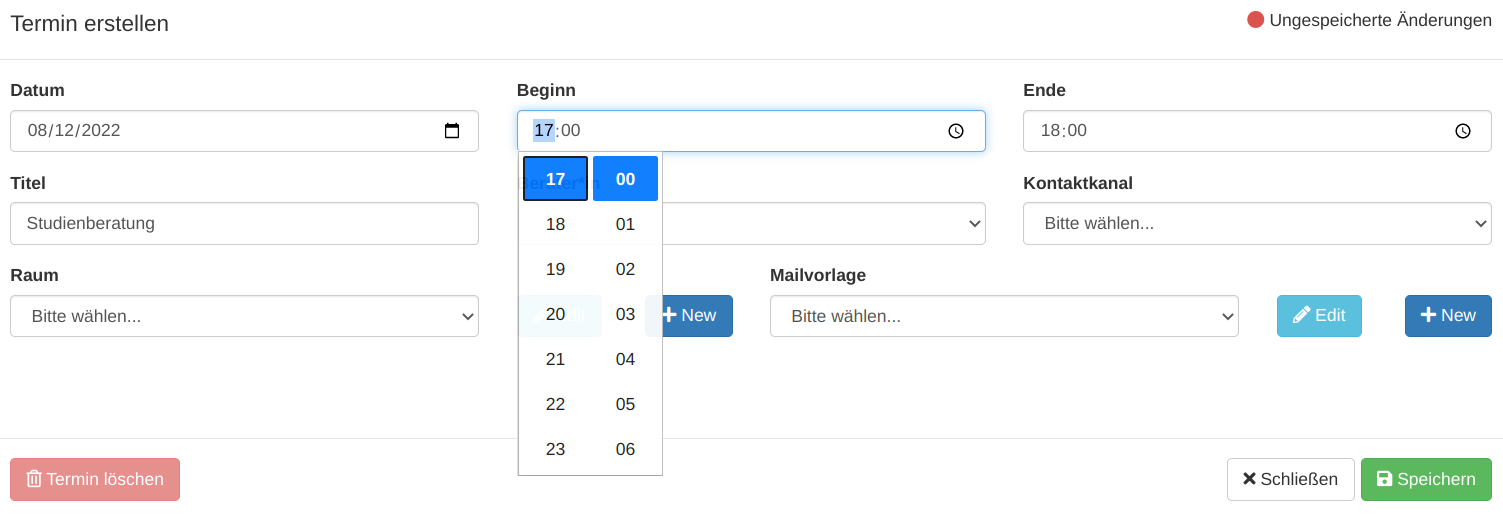
\includegraphics[width=0.9\textwidth]{screen_new_create_with_picker.png}
\end{figure}

Alle anderen Formularfelder füllt \ipName zügig aus. Da die abgefragten Daten
und die Anordnung der Eingabefelder genauso wie in der alten Version gestaltet
sind, merkt man hier, dass \ipName bereits viel Erfahrung mit der alten
Softwareversion von Stubegru gesammelt hat. Den unten rechts platzierten grünen
Button zum Speichern der Daten findet er sofort. Der Datensatz wird in der
Datenbank gespeichert und eine kleine grüne Meldung am linken unteren Rand
verkündet, dass der Termin erfolgreich gespeichert wurde. \ipName ist trotzdem
verunsichert, ob der Vorgang erfolgreich war. In der alten Version, hat sich
das Modal nach dem Speichern automatisch geschlossen. \ipName merkt an, dass in
der neuen Version nun jedes Mal ein zusätzlicher Klick auf den Button
\textit{Schließen} notwendig ist. Wenn das Modal sich nach dem Speichern direkt
schließen würde, wäre es für ihn einfacher. Ich erkläre, dass das Modal
geöffnet bleibt, damit ein neu erstellter Termin direkt an einen Kunden
vergeben werden kann. Nach dem Speichern erscheint hierfür der große blaue
Button mit der Aufschrift \textit{Termin vergeben}. \ipName erklärt, dass die
Termine eigentlich immer von den Hilfskräften der Erstinformation vergeben
werden und es für die Studienberatenden nicht nötig sei, den erstellten Termin
direkt vergeben zu können. Wir einigen uns darauf, dass ein Klick auf den
\textit{Speichern} Button das Modal, nach erfolgreichem Sichern der Daten,
schließt.

Und noch eine weitere Sache fällt \ipName auf: Wenn er bereits einen Termin
eingetragen hat und dann einen zweiten Termin erstellen möchte, werden alle
Eingabefelder zurückgesetzt und sind wieder leer. \glqq{}Das war in der alten
Version praktischer\grqq{}, sagt \ipName \glqq{}Oftmals trage ich viele Termine
für den gleichen Tag, mit den gleichen Attributen ein. Das einzige, was ich
bisher anpassen musste, war dann die Uhrzeit. Nun brauche ich viel mehr Klicks,
weil ich jedes Mal wieder den Raum und das Mailtemplate auswählen
muss.\grqq{}~\cite{clavesUsertest} Es stellt sich heraus, dass es in der alten
Softwareversion einen Bug gab, wodurch in einigen Fällen das Zurücksetzen des
Formulars nicht aufgerufen wurde. Dieser Bug hat sich in der Praxis dann
allerdings als sehr praktisch etabliert. Die Formularfelder nie zurückzusetzen
kann allerdings inkonsistente Status erzeugen, wenn zuvor beispielsweise ein
bereits vergebener Termin im Modal angezeigt wurde. Wir einigen uns auf eine
gemeinsame Idee: Wenn das Modal zum Erstellen eines Termins angezeigt wird,
erscheint in der Fußleiste ein weiterer Button mit der Aufschrift:
\textit{Speichern und nächster}. Dieser Button speichert den aktuellen Termin
und lässt das Modal ohne Zurücksetzen der Formularfelder geöffnet. Somit kann
direkt ein neuer Termin mit ähnlichen Attributen eingetragen werden.

\begin{figure}[H]
    \caption{Ein freier Termin. Studienberatende können Änderungen am Termin vornehmen oder einen Kunden einbuchen.}
    \centering
    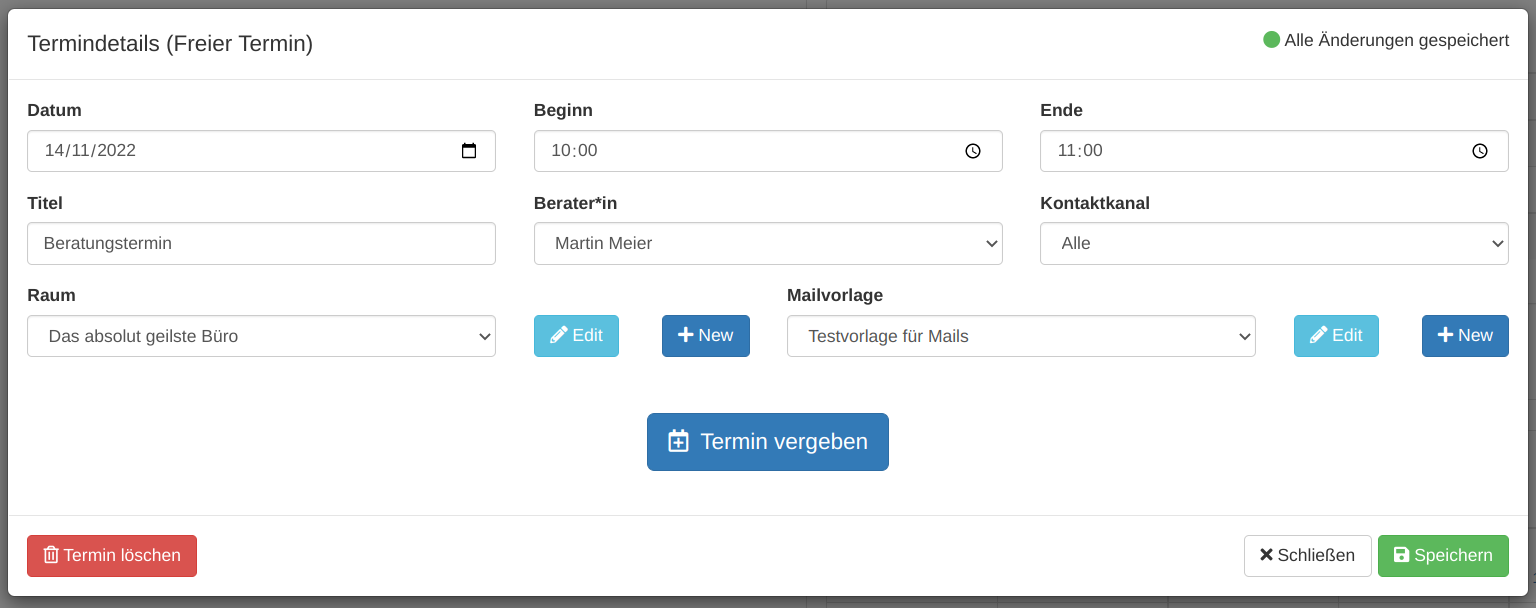
\includegraphics[width=0.9\textwidth]{screen_new_free_meeting.png}
\end{figure}

Als nächstes soll \ipName einen erstellten Zeitslot an einen Kunden vergeben.
Intuitiv klickt er hierfür auf den entsprechenden Termin in der
Monatsübersicht. Es öffnet sich das Modal mit der Detailansicht der
Termindaten. Sehr schnell findet \ipName den großen blauen Knopf zur
Terminvergabe. Wie er es bereits aus der alten Softwareversion kennt, öffnet
sich das Formular, um die weiteren Kundendaten einzutragen. \ipName prüft, was
passiert, wenn er hier relevante Felder einfach leer lässt. Beruhigt stellt er
fest, dass beim Versuch die Kundendaten zu speichern ein Hinweis am
entsprechenden leeren Eingabefeld auftaucht und das Speichern unvollständiger
Daten verhindert.

Nachdem alle Felder vollständig ausgefüllt sind, speichert \ipName die
Kundendaten und sieht eine leicht veränderte Detailansicht des Termins:

\begin{figure}[H]
    \caption{Ein vergebener Termin. Terminattribute und neue Kundendaten können erst nach Löschen der aktuellen Kundendaten hinterlegt werden.}
    \centering
    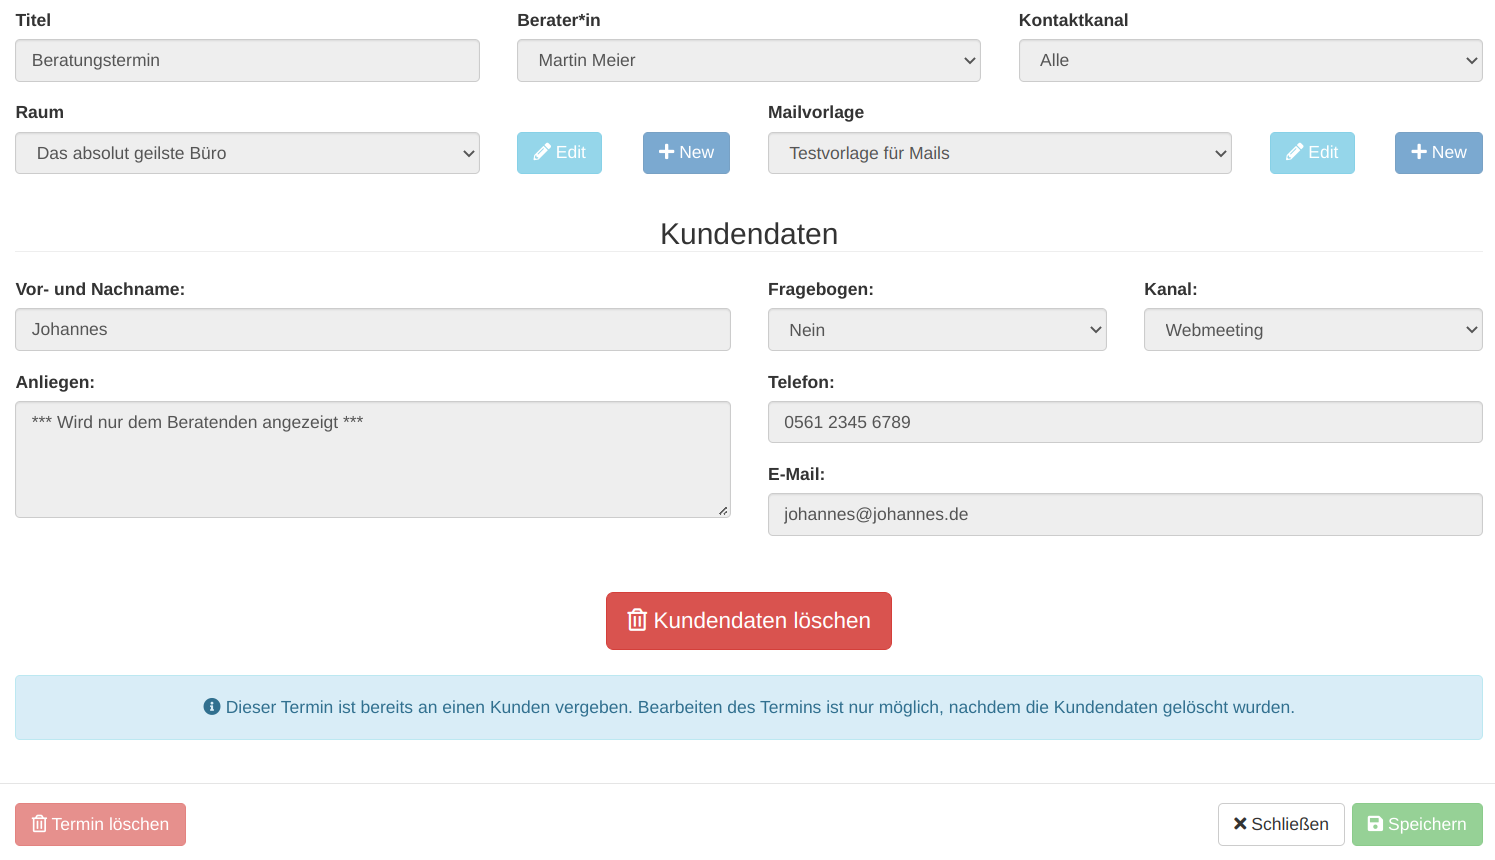
\includegraphics[width=0.9\textwidth]{screen_new_assigned.png}
\end{figure}

Die Terminattribute und Kundendaten können nicht weiter bearbeitet werden. Dies
erkennt \ipName schnell daran, dass die entsprechenden Eingabefelder ausgegraut
angezeigt werden. Zusätzlich verrät der Hinweis in der blauen Infobox, dass
Änderungen nur vorgenommen werden können, wenn zuvor die Kundendaten gelöscht
werden. \ipName realisiert, dass diese Einschränkung Sinn macht, da somit keine
Änderungen am Termin vorgenommen werden können, ohne dass der Kunde durch ein
erneutes Einbuchen darüber informiert wird.

\ipName freut sich, dass die Telefonnummer nun in übersichtlichen Blöcken von jeweils vier Ziffern angezeigt wird. Das Eintippen ins Telefon sei somit deutlich einfacher. Allerdings merkt er an, dass die Telefonnummer nur in dem Account des zugeordneten Beratenden angezeigt werden soll. So kann ein höherer Datenschutz gewährleistet werden und Hilfskräfte haben keinen Zugriff auf die Kontaktdaten aller ratsuchenden Kunden. Ich erkläre, dass ich diese Funktion bereits für das Beratungsanliegen umgesetzt habe. Wir loggen uns mit einem anderen Account ein und sehen, dass das Beratungsanliegen zensiert dargestellt wird. Diese Funktionalität soll in Zukunft auch für die Telefonnummer und Mailadresse der Kunden eingesetzt werden.

Abschließend betrachtet \ipName nochmals die Monatsübersicht. \glqq{}Wäre es
technisch aufwendig, bei den vergebenen, roten Terminen statt dem Namen des
Beratenden den Namen des Kunden anzuzeigen? So könnten die Hilfskräfte den
entsprechenden Termin eines Kunden schneller finden.\grqq{}, fragt er
mich~\cite{clavesUsertest}. Ich antworte, dass dies technisch kein großer
Aufwand wäre. Allerdings könnte es Verwirrung stiften, wenn bei manchen
Terminen der Name des Beratenden und bei anderen der Name des Kunden angezeigt
wird. Für den Fall, dass der Termin eines bestimmten Kunden schnell gefunden
werden muss, wurde außerdem die Suchfunktion entwickelt. \ipName erinnert sich
an die Suchfunktion und will diese direkt ausprobieren.

\begin{figure}[H]
    \caption{Suchfunktion, um bereits vergebene Termine anhand des eingebuchten Kunden zu finden. Die Suchanfrage \glqq{}jo\grqq{} ergibt drei Treffer.}
    \centering
    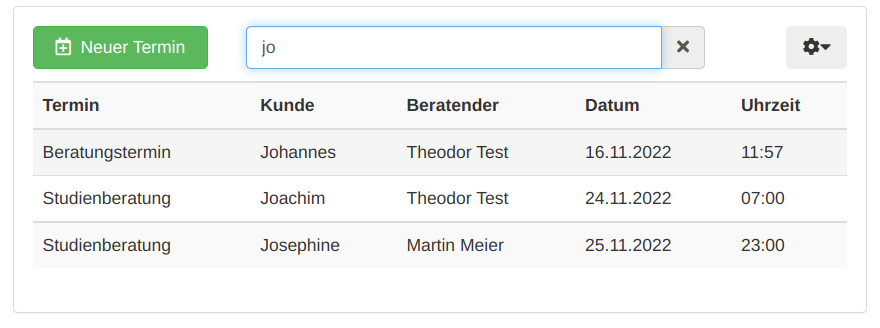
\includegraphics[width=0.9\textwidth]{screen_new_search.png}
\end{figure}

Das Eingabefeld für die Suchanfrage findet er schnell in der oberen
Navigationsleiste. Er gibt einige Buchstaben ein und direkt werden passende
Suchvorschläge angezeigt. \ipName ist überzeugt, dass dies eine gute Lösung
ist, um direkt nach Namen von ratsuchenden Kunden zu suchen. Er betont, dass es
wichtig ist, dass passenden Suchvorschläge bereits beim Tippen der ersten
Buchstaben angezeigt werden und kein Bestätigen der Suche mit Enter notwendig
ist.

Der Usertest ist nun beendet und \ipName bedankt sich für die entgegengebrachte
Aufmerksamkeit. Er ist sichtlich begeistert, dass die Nutzenden des Systems in
diesem Designprozess im Fokus stehen und freut sich auf die Einführung der
neuen Softwareversion: \glqq{}Wir müssen dann sicherlich eine Schulung für die
Hilfskräfte machen, um sie mit den neuen Features vertraut zu machen. Aber
eigentlich ist ja fast alles so, wie sie es schon gewohnt sind.\grqq{}, beendet
\ipName unser Gespräch~\cite{clavesUsertest}. Ich bedanke mich ebenfalls für die Zeit und die
konstruktive Kritik, die eine Diskussion über Verbesserungspotenziale erst
möglich gemacht hat.